\documentclass[mathserif]{beamer}

\usetheme[secheader]{Madrid}

\usepackage{tikz}
\usepackage{url}

\usepackage{pygments}
\usepackage{graphicx}

\providecommand{\code}[1]{{\texttt{\scriptsize{#1}}}}

\begin{document}

\section{The Problems}

\begin{frame}{The Challenge: A Flexible Interface to a Complex Model}
  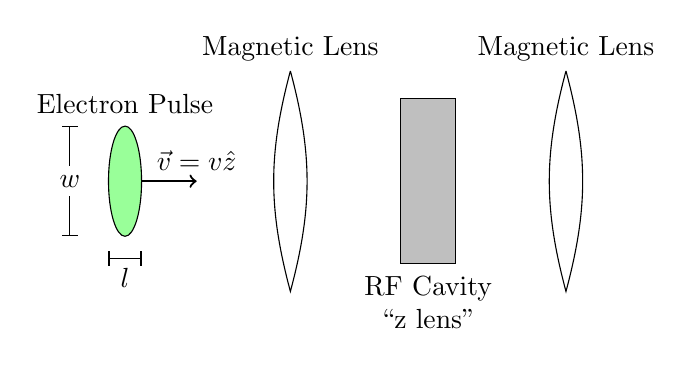
\begin{tikzpicture}[scale=0.7]
    \draw [fill=green!40] (0,0) ellipse [x radius=3mm, y radius=1cm];
    \draw [|-|] (-1,1) -- ++(0,-2) node [pos=0.5,fill=white] {$w$};
    \draw [|-|] (-0.3,-1.4) -- ++(0.6,0) node [pos=0.5,below] {$l$};
    \node at (0, 1.4) {Electron Pulse};
    \draw [thick, ->] (0.3,0) -- ++ (1,0) node [above,pos=1] {$\vec{v} = v \hat{z}$};
    \draw 
      (3,2)
      to [out=-75,in=75] ++(0,-4)
      to [out=105,in=255] ++(0,4)
      node [above] {Magnetic Lens}
    ;
    \draw [fill=gray!50] (5,1.5) rectangle ++(1,-3);
    \node at (5.5,-2.2) [align=center] {RF Cavity\\``z lens''};
    \draw 
      (8,2)
      to [out=-75,in=75] ++(0,-4)
      to [out=105,in=255] ++(0,4)
      node [above] {Magnetic Lens}
    ;
  \end{tikzpicture}
  \begin{itemize}
    \item Compute dynamics of electron pulse
    \item Generation and optical elements add terms to DE
  \end{itemize}
\end{frame}

\begin{frame}{The ``State of the Art''}
  Old codes are
  \begin{itemize}
    \item lacking full 6D dynamics
    \item optimized for performance vs usablilty
    \item hard to customize
    \item near impossible to comprehend
  \end{itemize}
  \begin{block}{\url{http://laacg.lanl.gov/laacg/services/download_sf.phtml}}
    \textbf{Getting Started with Poisson Superfish}\\
    \ldots We do not recommend trying to build an input file ``from scratch.'' Instead, find an example file that is similar to the problem you are trying to solve. Make a copy of the file and then make any necessary modifications to the geometry and options.
  \end{block}
\end{frame}

\begin{frame}{Physical Simulations}
  \begin{block}{Differential Equations}
    A set of rules that define how variables change with some parameter
    \begin{equation*}
      x(t_2) = x(t_1) + dt*\frac{dx}{dt}\visible<2->{(x,f(t1,t2))}
    \end{equation*}
  \end{block}
  \begin{block}{Example}
    \begin{equation*}
      \frac{dx}{dt} = -x \quad\implies\quad x(t) = sin(x*t) + C
    \end{equation*}
  \end{block}
\end{frame}

\begin{frame}{Other Attempts}
  \begin{columns}
    \begin{column}{0.49\linewidth}
      Mathematica:\\
      Pros:
      \begin{itemize}
        \item Can solve dynamics
        \item Pretty-printing of math for readability
      \end{itemize}
      Cons:
      \begin{itemize}
        \item Closed-source and expensive!
        \item No OO and no key-value datatypes
        \item Still rather slow $\sim$2mins$/$sim
      \end{itemize}
    \end{column}
    \begin{column}{0.49\linewidth}
      Modelica:\\
      Pros:
      \begin{itemize}
        \item Open-source, but behind close-source variants
        \item Unique OO language for physical simulation
        \item Classes have DEs as properties
      \end{itemize}
      Cons:
      \begin{itemize}
        \item Lacks ``has-a'' relationship
        \item Composing DEs not trivial
        \item User-facing object instantiation not trivial
        \item Some numerical problems (?)
      \end{itemize}
    \end{column}
  \end{columns}
\end{frame}

\section{Perl Solution}

\begin{frame}{\ldots But First, Some Bookkeeping}
  If an object knows where it is, can it remember where it came from?
  \begin{columns}
    \begin{column}{0.49\linewidth}
      \begin{block}{}
        \scriptsize
        \begin{Verbatim}[commandchars=\\\{\}]
\PY{k}{use} \PY{n+nn}{MooseX::Declare}\PY{p}{;}
\PY{k}{use} \PY{n+nn}{Method::Signatures::Modifiers}\PY{p}{;}
\PY{k}{use} \PY{n+nn}{MooseX::RememberHistory}\PY{p}{;}

\PY{n}{class} \PY{n}{MyClass} \PY{p}{\PYZob{}}
  \PY{n}{has} \PY{l+s}{'x'} \PY{o}{=}\PY{o}{>} \PY{p}{(} 
    \PY{n}{traits} \PY{o}{=}\PY{o}{>} \PY{p}{[}\PY{l+s}{'RememberHistory'}\PY{p}{]}\PY{p}{,} 
    \PY{n}{isa} \PY{o}{=}\PY{o}{>} \PY{l+s}{'Num'}\PY{p}{,} \PY{n}{is} \PY{o}{=}\PY{o}{>} \PY{l+s}{'rw'}\PY{p}{,}
    \PY{n}{default} \PY{o}{=}\PY{o}{>} \PY{l+m+mi}{0}
  \PY{p}{)}\PY{p}{;}
\PY{p}{\PYZcb{}}

\PY{k}{my} \PY{n+nv}{\PYZdl{}}\PY{n+nv}{obj} \PY{o}{=} \PY{n}{MyClass}\PY{o}{-}\PY{o}{>}\PY{k}{new}\PY{p}{;}
\PY{n+nv}{\PYZdl{}}\PY{n+nv}{obj}\PY{o}{-}\PY{o}{>}\PY{n}{x}\PY{p}{(} \PY{l+m+mi}{1} \PY{p}{)}\PY{p}{;}
\PY{n+nv}{\PYZdl{}}\PY{n+nv}{obj}\PY{o}{-}\PY{o}{>}\PY{n}{x}\PY{p}{(} \PY{l+m+mi}{2} \PY{p}{)}\PY{p}{;}

\PY{k}{print} \PY{n+nb}{join} \PY{l+s}{', '}\PY{p}{,} \PY{n+nv}{@}\PY{p}{\PYZob{}} \PY{n+nv}{\PYZdl{}}\PY{n+nv}{obj}\PY{o}{-}\PY{o}{>}\PY{n}{x\PYZus{}history} \PY{p}{\PYZcb{}}\PY{p}{;}
\PY{c+c1}{\PYZsh{} 0, 1, 2}
\end{Verbatim}

      \end{block}
    \end{column}
    \begin{column}{0.49\linewidth}
      \begin{itemize}
        \item works for fixed width solvers
        \item adaptive solvers call functions repeatedly (i.e. \code{PerlGSL::DiffEq})
          \begin{itemize}
            \item future work: attempt to add callbacks after finished step
          \end{itemize}
      \end{itemize}
    \end{column}
  \end{columns}
\end{frame}

\subsection{A Simple OO-DE Example}

\begin{frame}{The Solver: Attributes}
  \begin{block}{}
    \scriptsize
    \begin{Verbatim}[commandchars=\\\{\}]
\PY{n}{class} \PY{n}{MySim} \PY{p}{\PYZob{}}
  \PY{k}{use} \PY{n+nn}{List::Util} \PY{l+s}{'sum'}\PY{p}{;}

  \PY{n}{has} \PY{l+s}{'start'}  \PY{o}{=}\PY{o}{>} \PY{p}{(} \PY{n}{isa} \PY{o}{=}\PY{o}{>} \PY{l+s}{'Num'}\PY{p}{,} \PY{n}{is} \PY{o}{=}\PY{o}{>} \PY{l+s}{'ro'}\PY{p}{,} \PY{n}{default} \PY{o}{=}\PY{o}{>} \PY{l+m+mi}{0} \PY{p}{)}\PY{p}{;}
  \PY{n}{has} \PY{l+s}{'end'}    \PY{o}{=}\PY{o}{>} \PY{p}{(} \PY{n}{isa} \PY{o}{=}\PY{o}{>} \PY{l+s}{'Num'}\PY{p}{,} \PY{n}{is} \PY{o}{=}\PY{o}{>} \PY{l+s}{'ro'}\PY{p}{,} \PY{n}{default} \PY{o}{=}\PY{o}{>} \PY{l+m+mi}{1} \PY{p}{)}\PY{p}{;}
  \PY{n}{has} \PY{l+s}{'steps'}  \PY{o}{=}\PY{o}{>} \PY{p}{(} \PY{n}{isa} \PY{o}{=}\PY{o}{>} \PY{l+s}{'Num'}\PY{p}{,} \PY{n}{is} \PY{o}{=}\PY{o}{>} \PY{l+s}{'ro'}\PY{p}{,} \PY{n}{default} \PY{o}{=}\PY{o}{>} \PY{l+m+mi}{100} \PY{p}{)}\PY{p}{;}

  \PY{n}{has} \PY{l+s}{'step'}   \PY{o}{=}\PY{o}{>} \PY{p}{(} \PY{n}{isa} \PY{o}{=}\PY{o}{>} \PY{l+s}{'Num'}\PY{p}{,} \PY{n}{is} \PY{o}{=}\PY{o}{>} \PY{l+s}{'ro'}\PY{p}{,} \PY{n}{lazy} \PY{o}{=}\PY{o}{>} \PY{l+m+mi}{1}\PY{p}{,} \PY{n}{builder} \PY{o}{=}\PY{o}{>} \PY{l+s}{'init\PYZus{}step'}\PY{p}{)}\PY{p}{;}
  \PY{n}{has} \PY{l+s}{'time'}   \PY{o}{=}\PY{o}{>} \PY{p}{(} \PY{n}{traits} \PY{o}{=}\PY{o}{>} \PY{p}{[} \PY{l+s}{'RememberHistory'} \PY{p}{]}\PY{p}{,} \PY{n}{isa} \PY{o}{=}\PY{o}{>} \PY{l+s}{'Num'}\PY{p}{,} \PY{n}{is} \PY{o}{=}\PY{o}{>} \PY{l+s}{'rw'}\PY{p}{,} 
                    \PY{n}{lazy} \PY{o}{=}\PY{o}{>} \PY{l+m+mi}{1}\PY{p}{,} \PY{n}{builder} \PY{o}{=}\PY{o}{>} \PY{l+s}{'init\PYZus{}time'} \PY{p}{)}\PY{p}{;}

  \PY{n}{has} \PY{l+s}{'things'} \PY{o}{=}\PY{o}{>} \PY{p}{(} \PY{n}{isa} \PY{o}{=}\PY{o}{>} \PY{l+s}{'ArrayRef[MyThing]'}\PY{p}{,} \PY{n}{is} \PY{o}{=}\PY{o}{>} \PY{l+s}{'rw'}\PY{p}{,} \PY{n}{default} \PY{o}{=}\PY{o}{>} \PY{n}{sub}\PY{p}{\PYZob{}}\PY{o}{[]}\PY{p}{\PYZcb{}} \PY{p}{)}\PY{p}{;}
  \PY{n}{has} \PY{l+s}{'forces'} \PY{o}{=}\PY{o}{>} \PY{p}{(} \PY{n}{isa} \PY{o}{=}\PY{o}{>} \PY{l+s}{'ArrayRef[MyForce]'}\PY{p}{,} \PY{n}{is} \PY{o}{=}\PY{o}{>} \PY{l+s}{'rw'}\PY{p}{,} \PY{n}{default} \PY{o}{=}\PY{o}{>} \PY{n}{sub}\PY{p}{\PYZob{}}\PY{o}{[]}\PY{p}{\PYZcb{}} \PY{p}{)}\PY{p}{;}

  \PY{n}{method} \PY{n}{init\PYZus{}step} \PY{p}{(}\PY{p}{)} \PY{p}{\PYZob{}}
    \PY{k}{my} \PY{n+nv}{\PYZdl{}}\PY{n+nv}{step} \PY{o}{=} \PY{p}{(}\PY{n+nv}{\PYZdl{}}\PY{n+nv}{self}\PY{o}{-}\PY{o}{>}\PY{n}{end} \PY{o}{-} \PY{n+nv}{\PYZdl{}}\PY{n+nv}{self}\PY{o}{-}\PY{o}{>}\PY{n}{start}\PY{p}{)} \PY{o}{/} \PY{n+nv}{\PYZdl{}}\PY{n+nv}{self}\PY{o}{-}\PY{o}{>}\PY{n}{steps}\PY{p}{;}
    \PY{k}{return} \PY{n+nv}{\PYZdl{}}\PY{n+nv}{step}\PY{p}{;}
  \PY{p}{\PYZcb{}}

  \PY{n}{method} \PY{n}{init\PYZus{}time} \PY{p}{(}\PY{p}{)} \PY{p}{\PYZob{}} \PY{k}{return} \PY{n+nv}{\PYZdl{}}\PY{n+nv}{self}\PY{o}{-}\PY{o}{>}\PY{n}{start} \PY{p}{\PYZcb{}}
\end{Verbatim}

  \end{block}
\end{frame}

\begin{frame}{The Solver: Methods}
  \begin{block}{}
    \scriptsize
    \begin{Verbatim}[commandchars=\\\{\}]
  \PY{n}{method} \PY{n}{evolve} \PY{p}{(} \PY{n}{MyThing} \PY{n+nv}{\PYZdl{}}\PY{n+nv}{thing} \PY{p}{)} \PY{p}{\PYZob{}}
    \PY{k}{my} \PY{n+nv}{\PYZdl{}}\PY{n+nv}{dt} \PY{o}{=} \PY{n+nv}{\PYZdl{}}\PY{n+nv}{self}\PY{o}{-}\PY{o}{>}\PY{n}{step}\PY{p}{;}
    \PY{k}{my} \PY{n+nv}{\PYZdl{}}\PY{n+nv}{vx} \PY{o}{=} \PY{n+nv}{\PYZdl{}}\PY{n+nv}{thing}\PY{o}{-}\PY{o}{>}\PY{n}{vx}\PY{p}{;}

    \PY{k}{my} \PY{n+nv}{\PYZdl{}}\PY{n+nv}{force} \PY{o}{=} \PY{n}{sum} \PY{n+nb}{map} \PY{p}{\PYZob{}} \PY{n+nv}{\PYZdl{}}\PY{n+nv}{\PYZus{}}\PY{o}{-}\PY{o}{>}\PY{n}{affect}\PY{o}{-}\PY{o}{>}\PY{p}{(}\PY{n+nv}{\PYZdl{}}\PY{n+nv}{\PYZus{}}\PY{p}{,} \PY{n+nv}{\PYZdl{}}\PY{n+nv}{thing}\PY{p}{)} \PY{p}{\PYZcb{}} \PY{n+nv}{@}\PY{p}{\PYZob{}} \PY{n+nv}{\PYZdl{}}\PY{n+nv}{self}\PY{o}{-}\PY{o}{>}\PY{n}{forces} \PY{p}{\PYZcb{}}\PY{p}{;}
    \PY{k}{my} \PY{n+nv}{\PYZdl{}}\PY{n+nv}{acc} \PY{o}{=} \PY{n+nv}{\PYZdl{}}\PY{n+nv}{force} \PY{o}{/} \PY{p}{(}\PY{n+nv}{\PYZdl{}}\PY{n+nv}{thing}\PY{o}{-}\PY{o}{>}\PY{n}{mass}\PY{p}{)}\PY{p}{;}

    \PY{n+nv}{\PYZdl{}}\PY{n+nv}{thing}\PY{o}{-}\PY{o}{>}\PY{n}{vx}\PY{p}{(} \PY{n+nv}{\PYZdl{}}\PY{n+nv}{vx} \PY{o}{+} \PY{n+nv}{\PYZdl{}}\PY{n+nv}{acc} \PY{o}{*} \PY{n+nv}{\PYZdl{}}\PY{n+nv}{dt} \PY{p}{)}\PY{p}{;}
    \PY{n+nv}{\PYZdl{}}\PY{n+nv}{thing}\PY{o}{-}\PY{o}{>}\PY{n}{x}\PY{p}{(} \PY{n+nv}{\PYZdl{}}\PY{n+nv}{thing}\PY{o}{-}\PY{o}{>}\PY{n}{x} \PY{o}{+} \PY{n+nv}{\PYZdl{}}\PY{n+nv}{vx} \PY{o}{*} \PY{n+nv}{\PYZdl{}}\PY{n+nv}{dt} \PY{p}{)}\PY{p}{;}
  \PY{p}{\PYZcb{}}

  \PY{n}{method} \PY{n}{run} \PY{p}{(}\PY{p}{)} \PY{p}{\PYZob{}}
    \PY{k}{while} \PY{p}{(}\PY{n+nv}{\PYZdl{}}\PY{n+nv}{self}\PY{o}{-}\PY{o}{>}\PY{n+nb}{time} \PY{o}{<} \PY{n+nv}{\PYZdl{}}\PY{n+nv}{self}\PY{o}{-}\PY{o}{>}\PY{n}{end}\PY{p}{)} \PY{p}{\PYZob{}}
      \PY{n+nv}{\PYZdl{}}\PY{n+nv}{self}\PY{o}{-}\PY{o}{>}\PY{n}{evolve}\PY{p}{(} \PY{n+nv}{\PYZdl{}}\PY{n+nv}{\PYZus{}} \PY{p}{)} \PY{k}{for} \PY{n+nv}{@}\PY{p}{\PYZob{}} \PY{n+nv}{\PYZdl{}}\PY{n+nv}{self}\PY{o}{-}\PY{o}{>}\PY{n}{things} \PY{p}{\PYZcb{}}\PY{p}{;}
      \PY{n+nv}{\PYZdl{}}\PY{n+nv}{self}\PY{o}{-}\PY{o}{>}\PY{n+nb}{time}\PY{p}{(} \PY{n+nv}{\PYZdl{}}\PY{n+nv}{self}\PY{o}{-}\PY{o}{>}\PY{n+nb}{time} \PY{o}{+} \PY{n+nv}{\PYZdl{}}\PY{n+nv}{self}\PY{o}{-}\PY{o}{>}\PY{n}{step} \PY{p}{)}\PY{p}{;}
    \PY{p}{\PYZcb{}}
  \PY{p}{\PYZcb{}}
\PY{p}{\PYZcb{}} \PY{c+c1}{\PYZsh{} end of class MySim}
\end{Verbatim}

  \end{block}
\end{frame}

\begin{frame}{Physical Classes}
  \begin{block}{}
    \scriptsize
    \begin{Verbatim}[commandchars=\\\{\}]
\PY{n}{class} \PY{n}{MyForce} \PY{p}{\PYZob{}}

  \PY{n}{has} \PY{l+s}{'strength'} \PY{o}{=}\PY{o}{>} \PY{p}{(} \PY{n}{isa} \PY{o}{=}\PY{o}{>} \PY{l+s}{'Num'}\PY{p}{,}  \PY{n}{is} \PY{o}{=}\PY{o}{>} \PY{l+s}{'rw'}\PY{p}{,} \PY{n}{default} \PY{o}{=}\PY{o}{>} \PY{l+m+mi}{0} \PY{p}{)}\PY{p}{;}
  \PY{n}{has} \PY{l+s}{'affect'}   \PY{o}{=}\PY{o}{>} \PY{p}{(} \PY{n}{isa} \PY{o}{=}\PY{o}{>} \PY{l+s}{'CodeRef'}\PY{p}{,} \PY{n}{is} \PY{o}{=}\PY{o}{>} \PY{l+s}{'ro'}\PY{p}{,} \PY{n}{required} \PY{o}{=}\PY{o}{>} \PY{l+m+mi}{1} \PY{p}{)}\PY{p}{;}
  
\PY{p}{\PYZcb{}}

\PY{n}{class} \PY{n}{MyThing} \PY{p}{\PYZob{}}

  \PY{n}{has} \PY{l+s}{'mass'} \PY{o}{=}\PY{o}{>} \PY{p}{(} \PY{n}{isa} \PY{o}{=}\PY{o}{>} \PY{l+s}{'Num'}\PY{p}{,} \PY{n}{is} \PY{o}{=}\PY{o}{>} \PY{l+s}{'ro'}\PY{p}{,} \PY{n}{required} \PY{o}{=}\PY{o}{>} \PY{l+m+mi}{1} \PY{p}{)}\PY{p}{;}
  \PY{n}{has} \PY{l+s}{'x'}    \PY{o}{=}\PY{o}{>} \PY{p}{(} \PY{n}{traits} \PY{o}{=}\PY{o}{>} \PY{p}{[} \PY{l+s}{'RememberHistory'} \PY{p}{]}\PY{p}{,} \PY{n}{isa} \PY{o}{=}\PY{o}{>} \PY{l+s}{'Num'}\PY{p}{,} 
                  \PY{n}{is} \PY{o}{=}\PY{o}{>} \PY{l+s}{'rw'}\PY{p}{,} \PY{n}{default} \PY{o}{=}\PY{o}{>} \PY{l+m+mi}{0} \PY{p}{)}\PY{p}{;}
  \PY{n}{has} \PY{l+s}{'vx'}   \PY{o}{=}\PY{o}{>} \PY{p}{(} \PY{n}{traits} \PY{o}{=}\PY{o}{>} \PY{p}{[} \PY{l+s}{'RememberHistory'} \PY{p}{]}\PY{p}{,} \PY{n}{isa} \PY{o}{=}\PY{o}{>} \PY{l+s}{'Num'}\PY{p}{,}
                  \PY{n}{is} \PY{o}{=}\PY{o}{>} \PY{l+s}{'rw'}\PY{p}{,} \PY{n}{default} \PY{o}{=}\PY{o}{>} \PY{l+m+mi}{0} \PY{p}{)}\PY{p}{;}

\PY{p}{\PYZcb{}}
\end{Verbatim}

  \end{block}
\end{frame}

\begin{frame}{The Script}
  \begin{columns}
    \begin{column}{0.49\linewidth}
      \begin{block}{}
        \scriptsize
        \begin{Verbatim}[commandchars=\\\{\}]
\PY{c+c1}{\PYZsh{}!/usr/bin/env perl}
\PY{k}{use} \PY{n}{strict}\PY{p}{;} \PY{k}{use} \PY{n}{warnings}\PY{p}{;}
\PY{k}{use} \PY{n+nn}{MySim}\PY{p}{;}
\PY{k}{use} \PY{n+nn}{PDL}\PY{p}{;}
\PY{k}{use} \PY{n+nn}{PDL::}\PY{n+nn}{Graphics::Prima::Simple}\PY{p}{;}

\PY{k}{my} \PY{n+nv}{\PYZdl{}}\PY{n+nv}{thing} \PY{o}{=} \PY{n}{MyThing}\PY{o}{-}\PY{o}{>}\PY{k}{new}\PY{p}{(} \PY{n}{mass} \PY{o}{=}\PY{o}{>} \PY{l+m+mi}{2} \PY{p}{)}\PY{p}{;}

\PY{k}{my} \PY{n+nv}{\PYZdl{}}\PY{n+nv}{acc} \PY{o}{=} \PY{n}{MyForce}\PY{o}{-}\PY{o}{>}\PY{k}{new}\PY{p}{(}
  \PY{n}{strength} \PY{o}{=}\PY{o}{>} \PY{l+m+mi}{2}\PY{p}{,}
  \PY{n}{affect} \PY{o}{=}\PY{o}{>} \PY{k}{sub }\PY{p}{\PYZob{}}\PY{n+nb}{shift}\PY{o}{-}\PY{o}{>}\PY{n}{strength}\PY{p}{\PYZcb{}}\PY{p}{,}
\PY{p}{)}\PY{p}{;}

\PY{k}{my} \PY{n+nv}{\PYZdl{}}\PY{n+nv}{dec} \PY{o}{=} \PY{n}{MyForce}\PY{o}{-}\PY{o}{>}\PY{k}{new}\PY{p}{(}
  \PY{n}{strength} \PY{o}{=}\PY{o}{>} \PY{o}{-}\PY{l+m+mi}{50}\PY{p}{,}
  \PY{n}{affect} \PY{o}{=}\PY{o}{>} \PY{k}{sub }\PY{p}{\PYZob{}}
    \PY{k}{my} \PY{p}{(}\PY{n+nv}{\PYZdl{}}\PY{n+nv}{self}\PY{p}{,} \PY{n+nv}{\PYZdl{}}\PY{n+nv}{thing}\PY{p}{)} \PY{o}{=} \PY{n+nv}{@}\PY{n+nv}{\PYZus{}}\PY{p}{;}
    \PY{k}{return} \PY{l+m+mi}{0} \PY{k}{if} \PY{p}{(}\PY{n+nv}{\PYZdl{}}\PY{n+nv}{thing}\PY{o}{-}\PY{o}{>}\PY{n}{x} \PY{o}{<} \PY{l+m+mf}{0.1}\PY{p}{)}\PY{p}{;}
    \PY{k}{return} \PY{n+nv}{\PYZdl{}}\PY{n+nv}{self}\PY{o}{-}\PY{o}{>}\PY{n}{strength}\PY{p}{;}
  \PY{p}{\PYZcb{}}\PY{p}{,}
\PY{p}{)}\PY{p}{;}
\end{Verbatim}

      \end{block}
    \end{column}
    \begin{column}{0.49\linewidth}
      \begin{block}{}
        \scriptsize
        \begin{Verbatim}[commandchars=\\\{\}]
\PY{k}{my} \PY{n+nv}{\PYZdl{}}\PY{n+nv}{sim} \PY{o}{=} \PY{n}{MySim}\PY{o}{-}\PY{o}{>}\PY{k}{new}\PY{p}{(}
  \PY{n}{end} \PY{o}{=}\PY{o}{>} \PY{l+m+mi}{5}\PY{p}{,}
  \PY{n}{things} \PY{o}{=}\PY{o}{>} \PY{p}{[} \PY{n+nv}{\PYZdl{}}\PY{n+nv}{thing} \PY{p}{]}\PY{p}{,}
  \PY{n}{forces} \PY{o}{=}\PY{o}{>} \PY{p}{[} \PY{n+nv}{\PYZdl{}}\PY{n+nv}{acc}\PY{p}{,} \PY{n+nv}{\PYZdl{}}\PY{n+nv}{dec} \PY{p}{]}\PY{p}{,}
\PY{p}{)}\PY{p}{;}

\PY{n+nv}{\PYZdl{}}\PY{n+nv}{sim}\PY{o}{-}\PY{o}{>}\PY{n}{run}\PY{p}{;}

\PY{k}{my} \PY{n+nv}{\PYZdl{}}\PY{n+nv}{time} \PY{o}{=} \PY{n}{pdl} \PY{n+nv}{\PYZdl{}}\PY{n+nv}{sim}\PY{o}{-}\PY{o}{>}\PY{n}{time\PYZus{}history}\PY{p}{;}
\PY{k}{my} \PY{n+nv}{\PYZdl{}}\PY{n+nv}{x}    \PY{o}{=} \PY{n}{pdl} \PY{n+nv}{\PYZdl{}}\PY{n+nv}{thing}\PY{o}{-}\PY{o}{>}\PY{n}{x\PYZus{}history}\PY{p}{;}

\PY{n}{line\PYZus{}plot}\PY{p}{(}\PY{n+nv}{\PYZdl{}}\PY{n+nv}{time}\PY{p}{,} \PY{n+nv}{\PYZdl{}}\PY{n+nv}{x}\PY{p}{)}\PY{p}{;}
\end{Verbatim}

      \end{block}
      \centering
      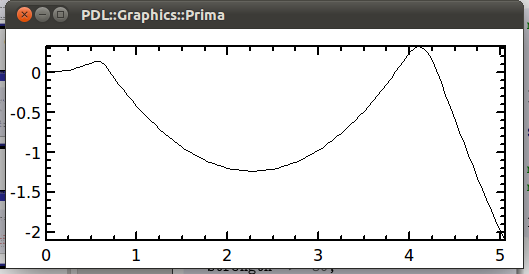
\includegraphics[width=0.8\linewidth]{example.png}
    \end{column}
  \end{columns}
\end{frame}

\section{Units Handling}

\begin{frame}{Unit Handling (The Implied Covenant)}
  \begin{block}{Mars Surveyor '98 Orbiter (Sorry Larry!)}
    \begin{itemize}
      \item Software used force in Newtons
      \item Users entered force in Foot-Pounds
    \end{itemize}
  \end{block}
  \vfill
  The Covenant:
  \begin{itemize}
    \item Between programmer and user
    \item ``Use the same units!''
    \item Unexpected and possibly undocumented action at a distance
    \item With Perl and Moose we can do better \ldots
  \end{itemize}
\end{frame}

\begin{frame}{\texttt{MooseX::Types::NumUnit}}
  \begin{itemize}
    \item \code{Str} to \code{Num} coercions
    \item convert unit if needed
  \end{itemize}
  \begin{block}{}
    \scriptsize
    \begin{Verbatim}[commandchars=\\\{\}]
\PY{k}{use} \PY{n+nn}{MooseX::Declare}\PY{p}{;}
\PY{k}{use} \PY{n+nn}{Method::Signatures::Modifiers}\PY{p}{;}

\PY{n}{class} \PY{n}{SphericalCow} \PY{p}{\PYZob{}}
  \PY{k}{use} \PY{n+nn}{MooseX::Types::NumUnit} \PY{l+s+sx}{qw/num\PYZus{}of\PYZus{}unit/}\PY{p}{;}
  \PY{n}{has} \PY{l+s}{'radius'}   \PY{o}{=}\PY{o}{>} \PY{p}{(} \PY{n}{isa} \PY{o}{=}\PY{o}{>} \PY{n}{num\PYZus{}of\PYZus{}unit}\PY{p}{(}\PY{l+s}{'m'}\PY{p}{)}\PY{p}{,}   \PY{n}{is} \PY{o}{=}\PY{o}{>} \PY{l+s}{'rw'}\PY{p}{,} \PY{n}{default} \PY{o}{=}\PY{o}{>} \PY{l+m+mi}{1} \PY{p}{)}\PY{p}{;}
  \PY{n}{has} \PY{l+s}{'velocity'} \PY{o}{=}\PY{o}{>} \PY{p}{(} \PY{n}{isa} \PY{o}{=}\PY{o}{>} \PY{n}{num\PYZus{}of\PYZus{}unit}\PY{p}{(}\PY{l+s}{'m/s'}\PY{p}{)}\PY{p}{,} \PY{n}{is} \PY{o}{=}\PY{o}{>} \PY{l+s}{'rw'}\PY{p}{,} \PY{n}{default} \PY{o}{=}\PY{o}{>} \PY{l+m+mi}{0} \PY{p}{)}\PY{p}{;}
\PY{p}{\PYZcb{}}

\PY{k}{use} \PY{n}{strict}\PY{p}{;} \PY{k}{use} \PY{n}{warnings}\PY{p}{;}

\PY{k}{my} \PY{n+nv}{\PYZdl{}}\PY{n+nv}{cow} \PY{o}{=} \PY{n}{SphericalCow}\PY{o}{-}\PY{o}{>}\PY{k}{new}\PY{p}{(}
  \PY{n}{radius} \PY{o}{=}\PY{o}{>} \PY{l+s}{'1 ft'}\PY{p}{,}
\PY{p}{)}\PY{p}{;}

\PY{k}{print} \PY{n+nv}{\PYZdl{}}\PY{n+nv}{cow}\PY{o}{-}\PY{o}{>}\PY{n}{radius} \PY{o}{.} \PY{l+s}{"\PYZbs{}n"}\PY{p}{;} \PY{c+c1}{\PYZsh{} 0.3048}
\end{Verbatim}

  \end{block}
\end{frame}

\begin{frame}{Example of \texttt{Physics::UEMColumn}}
  Back to the original problem of Electron Column Modeling
  \begin{itemize}
    \item As yet unreleased \code{Physics::UEMColumn}
    \begin{itemize}
      \item \url{https://github.com/jberger/Physics-UEMColumn}
    \end{itemize}
    \item Uses: \code{PerlGSL::DiffEq} on CPAN
    \begin{itemize}
      \item C-level solver of Perl-level DE closures
    \end{itemize}
  \end{itemize}
\end{frame}

\end{document}
